\clearpage\begingroup
\SourceLeaf{137b}\HistoricalHead{132}{L}{PHYSIK.\quad NACHLASS.}
\newcommand{\IVdoublebar}[1]{\overline{\overline{#1}}}
\begin{center}\textbf{ERLÄUTERUNGEN.}\end{center}
\noindent\hspace*{\parindent}Die hier gestellte Aufgabe, die $\alpha',\beta',\mu',\nu'$ aus den $\alpha,\beta,\mu,\nu$ zu bestimmen, ist die auch in den »\textit{Dioptrischen Untersuchungen}« vorliegende (Werke V, S. 246 ff.); sie wird hier anders gelöst, als dort.

Der hier zuerst behandelte Spezialfall $\mu=\nu=0$ bedeutet, daß der einfallende Strahl parallel der $x$-Achse (d.\,h. der Achse des optischen Systems) eintritt; bezieht man sich auf die folgende Figur, die in der Ebene der $x$ und $\rho=\sqrt{y^2+z^2}$, d.\,h. der Ebene des einfallenden und gebrochenen Strahles, gezeichnet ist, so hat man offenbar folgendes:
\begin{center}
\begin{tikzpicture}[x=.012cm,y=-.012cm,line width=.6pt,font=\small]
\draw[->] (160,246)--(1095,246);
\draw[->] (595,430)--(595,22);
\node[right] at (1095,246) {$x$};
\node[right] at (610,23) {$\rho=\sqrt{z^2+y^2}$};
\draw (40,145)--(415,145);
\draw[->] (140,145)--(205,145);
\draw (303,84)--(595,246);
\draw (415,145)--(870,246);
\draw (415,145)--(415,246);
\draw (445,108)..controls (370,190) and (375,308)..(450,388);
\node[above right] at (418,143) {$B$};
\node[above right] at (870,244) {$C$};
\node[right] at (415,193) {$\IVdoublebar\rho$};
\draw (369,145)..controls (369,138) and (372,132)..(375,123);
\node at (348,125) {$\vartheta$};
\draw (539,246)..controls (539,236) and (541,229)..(546,219);
\node at (523,228) {$\vartheta$};
\draw (469,157)..controls (469,163) and (467,169)..(463,172);
\draw (476,159)..controls (476,166) and (473,173)..(469,176);
\node at (497,176) {$\varepsilon$};
\draw (786,246)..controls (786,240) and (787,235)..(790,228);
\draw (792,246)..controls (792,240) and (793,235)..(796,230);
\draw (798,246)..controls (798,241) and (799,236)..(802,231);
\node at (750,233) {$\sigma$};
\draw (415,246)..controls (415,265) and (431,265)..(447,265)--(475,265)
 ..controls (488,265) and (495,272)..(500,282)
 ..controls (504,272) and (511,265)..(525,265)--(563,265)
 ..controls (581,265) and (594,260)..(595,246);
\node[below] at (500,283) {$\IVdoublebar x$};
\draw (595,246)..controls (596,264) and (621,265)..(641,265)--(696,265)
 ..controls (716,265) and (729,274)..(733,284)
 ..controls (737,274) and (748,265)..(768,265)--(833,265)
 ..controls (853,265) and (867,260)..(870,246);
\node[below] at (733,285) {$\bar x$};
\end{tikzpicture}
\end{center}
\noindent\hspace*{\parindent}Die Koordinaten des Punktes $B$, in dem der einfallende Strahl die Kugelfläche trifft, sind $\IVdoublebar\rho=\sqrt{\alpha^2+\beta^2}$, gemäß der Bedingung, daß für den einfallenden Strahl $\mu=\nu=0$ sind, und $\IVdoublebar x=\sqrt{r^2-\alpha^2-\beta^2}$, da $B$ gleichzeitig auf dem Kreise $x^2+\rho^2=r^2$ liegt. Also erhält man für den Kosinus und Sinus des spitzen Winkels $\vartheta$ die Werte:
\[
\cos\vartheta=\frac{\sqrt{r^2-\alpha^2-\beta^2}}r,\qquad
\sin\vartheta=\frac{\sqrt{\alpha^2+\beta^2}}r.
\]
\noindent Nach dem Brechungsgesetz ist
\[
\frac{\sin\vartheta}n=\sin\varepsilon,
\]
\noindent und daher folgt für den spitzen Winkel $\varepsilon$:
\[
\sin\varepsilon=\frac{\sqrt{\alpha^2+\beta^2}}{nr},\qquad
\cos\varepsilon=\frac{\sqrt{n^2r^2-\alpha^2-\beta^2}}{nr}.
\]
\clearpage\SourceLeaf{138}\HistoricalHead{133}{R}{AUFGABE AUS DER DIOPTRIK.}
\noindent Endlich ist der spitze Winkel $\sigma$, den der gebrochene Strahl mit der $x$-Achse bildet, gleich $\vartheta-\varepsilon$, also:
\[
\sin\sigma=\sin(\vartheta-\varepsilon)
=\frac{\sqrt{\alpha^2+\beta^2}\{\sqrt{n^2r^2-\alpha^2-\beta^2}-\sqrt{r^2-\alpha^2-\beta^2}\}}{nr^2},
\]
\noindent also nach dem Sinussatze
\[
\bar x=r\frac{\sin\varepsilon}{\sin\sigma}
=\frac{r^2}{\sqrt{n^2r^2-\alpha^2-\beta^2}-\sqrt{r^2-\alpha^2-\beta^2}},
\]
\noindent oder
\[
\bar x=\frac{\sqrt{n^2r^2-\alpha^2-\beta^2}+\sqrt{r^2-\alpha^2-\beta^2}}{n^2-1},
\]
\noindent was genau der von \textsc{Gauss} angegebene Wert ist. Die Koordinaten des Punktes $C$, in dem der gebrochene Strahl die Achse trifft, sind also folgende:
\[
\bar x=\frac{\sqrt{n^2r^2-\alpha^2-\beta^2}+\sqrt{r^2-\alpha^2-\beta^2}}{n^2-1},\qquad \bar\rho=0,
\]
\noindent d.\,h. $\bar y=\bar z=0$.

Setzt man nun an, daß die Ebene
\[
y=\alpha'+\mu'x
\]
\noindent durch die beiden Punkte $B$ und $C$ hindurchgeht, so erhält man ohne weiteres die von \textsc{Gauss} im Texte angegebenen Werte für $\alpha'$ und $\mu'$ und entsprechend für $\beta'$ und $\gamma'$.

Der zweite Spezialfall ist durch $\beta=\nu=0$ charakterisiert, d.\,h. die Ebene des einfallenden und gebrochenen Strahles ist mit der $xy$-Ebene zusammenfallend gedacht, was übrigens in keiner Weise eine Beschränkung der Allgemeinheit ist. Wir haben dann folgende Figur:
\begin{center}
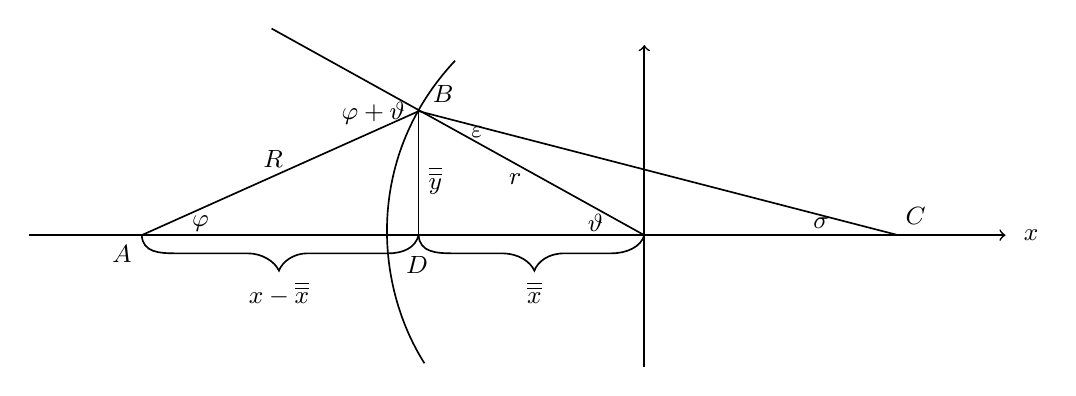
\begin{tikzpicture}[x=.0105cm,y=-.0105cm,line width=.6pt,font=\small]
\draw[->] (28,280)--(1210,280);
\draw[->] (773,439)--(773,50);
\node[right] at (1220,280) {$x$};
\draw (165,280)--(500,130);
\draw (322,30)--(773,280);
\draw (500,130)--(1080,280);
\draw (500,130)--(500,280);
\draw (544,69)..controls (437,183) and (445,337)..(507,435);
\node[below left] at (165,280) {$A$};
\node[above right] at (505,132) {$B$};
\node[above right] at (1077,279) {$C$};
\node[below] at (498,294) {$D$};
\node[right] at (500,214) {$\IVdoublebar y$};
\node at (324,188) {$R$};
\node at (617,212) {$r$};
\node at (236,266) {$\varphi$};
\node at (445,132) {$\varphi+\vartheta$};
\node at (571,155) {$\varepsilon$};
\node at (714,265) {$\vartheta$};
\node at (987,265) {$\sigma$};
\draw (165,280)..controls (166,301) and (187,302)..(205,302)--(293,302)
 ..controls (311,302) and (326,312)..(331,323)
 ..controls (335,312) and (349,302)..(365,302)--(463,302)
 ..controls (482,302) and (496,295)..(500,280);
\node[below] at (331,324) {$x-\IVdoublebar x$};
\draw (500,280)..controls (501,301) and (522,302)..(542,302)--(600,302)
 ..controls (621,302) and (635,312)..(640,323)
 ..controls (644,312) and (657,302)..(676,302)--(733,302)
 ..controls (752,302) and (769,294)..(773,280);
\node[below] at (640,324) {$\IVdoublebar x$};
\end{tikzpicture}
\end{center}
\noindent Zunächst erhält man für die Koordinaten $\IVdoublebar x,\IVdoublebar y$ des Schnittpunktes $B$ des einfallenden Strahls mit der Kugelfläche die Werthe
\[
\IVdoublebar x=-\frac{\alpha\mu+P}{1+\mu^2},\qquad
\IVdoublebar y=\frac{\alpha-\mu P}{1+\mu^2},
\]
\noindent wo $P$ die von \textsc{Gauss} benützte Abkürzung für $\sqrt{(1+\mu^2)r^2-\alpha^2}$ ist.

Die Koordinaten $x,y$ des Punktes $A$, in dem der einfallende Strahl die Abszissenachse schneidet, sind offenbar:
\[
x=-\frac\alpha\mu,\qquad y=0,
\]
\noindent also folgt für die Strecke $AB=R$ der Wert
\[
R=\frac{\alpha-\mu P}{\mu\sqrt{1+\mu^2}}.
\]
\clearpage\SourceLeaf{139}\HistoricalHead{134}{L}{PHYSIK.\quad NACHLASS.}
\noindent Es ergeben sich dann der Reihe nach folgende Werte für Kosinus und Sinus der Winkel $\vartheta,\varphi,\varepsilon,\sigma$, deren Beziehungen aus der Figur abzulesen sind:
\[
\begin{aligned}
\cos\vartheta&=\frac{\alpha\mu+P}{r(1+\mu^2)},&\sin\vartheta&=\frac{\alpha-\mu P}{r(1+\mu^2)},\\[6pt]
\cos\varphi&=\frac1{\sqrt{1+\mu^2}},&\sin\varphi&=\frac\mu{\sqrt{1+\mu^2}},\\[6pt]
\cos\varepsilon&=\frac Q{nr\sqrt{1+\mu^2}},&\sin\varepsilon&=\frac\alpha{nr\sqrt{1+\mu^2}},
\end{aligned}
\]
\[
\begin{aligned}
\cos\sigma&=\frac{Q(\alpha\mu+P)+\alpha(\alpha-\mu P)}{nr^2(1+\mu^2)\sqrt{1+\mu^2}},\\[6pt]
\sin\sigma&=\frac{Q(\alpha-\mu P)-\alpha(\alpha\mu+P)}{nr^2(1+\mu^2)\sqrt{1+\mu^2}};
\end{aligned}
\]
\noindent also folgt schließlich für $\operatorname{tg}\sigma$, das definitionsgemäß gleich $-\mu'$ ist,
\[
-\mu'=\operatorname{tg}\sigma=\frac{Q(\alpha-\mu P)-\alpha(\alpha\mu+P)}{Q(\alpha\mu+P)+\alpha(\alpha-\mu P)},
\]
\noindent worin $Q$ wie im Texte gleich $\sqrt{(1+\mu^2)n^2r^2-\alpha^2}$ zu nehmen ist. Setzt man darin die Werte ein, so folgt der von \textsc{Gauss} angegebene Wert für $\mu'$, und aus diesem sofort derjenige von $\alpha'$.

Die gestellte Aufgabe ist damit gelöst.
\begin{flushright}\textsc{Schaefer.}\end{flushright}
\begin{center}\rule{.25\linewidth}{.4pt}\end{center}
\clearpage\endgroup
